\chapter{Architecture}
\label{ch:arch}

\section{Layers}

\begin{figure}[h]
  \centering
  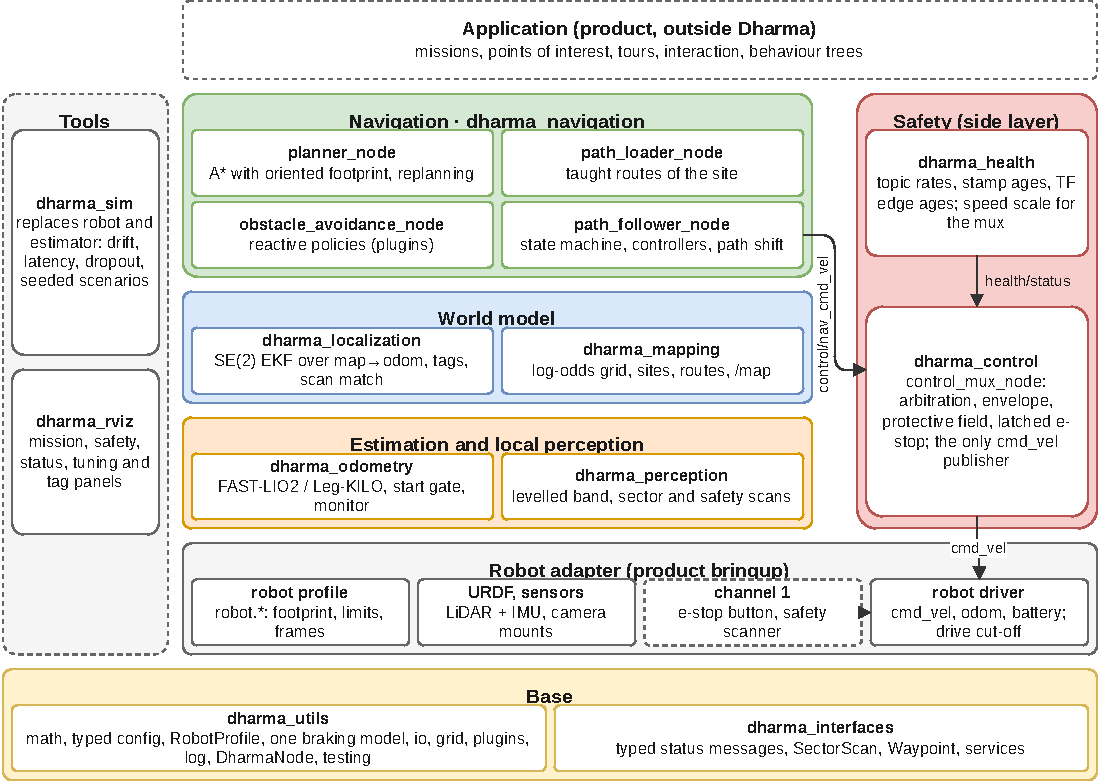
\includegraphics[width=\textwidth]{layers}
  \caption{Layers of Dharma. Colours: estimation orange, world model blue, navigation green,
    safety red, base yellow, hardware grey.}
  \label{fig:layers}
\end{figure}

Dharma is organised in layers (Fig.~\ref{fig:layers}); each depends only on the layers below and
on the base packages.

\begin{description}
  \item[Robot adapter] (product). The driver bridge (velocity command in, robot odometry and
    battery out), the URDF with the sensor mounts, and the robot profile. A hardware e-stop and,
    where required, a safety-rated scanner act on the drive directly (channel~1,
    Section~\ref{sec:two-channel}).
  \item[Estimation and local perception.] \pkg{dharma_odometry} runs a LiDAR-inertial estimator
    and monitors it; \pkg{dharma_perception} turns the LiDAR into obstacle sectors around the
    robot and throttles the camera for the fiducial detector.
  \item[World model.] \pkg{dharma_localization} keeps \frm{map}$\to$\frm{odom} from fiducials,
    operator input and optional scan matching; \pkg{dharma_mapping} records occupancy maps and
    manages sites and routes.
  \item[Navigation.] \pkg{dharma_navigation} plans on the map, loads taught routes, follows
    paths and runs reactive avoidance. Its velocity output is \topic{control/nav_cmd_vel},
    never the robot's \topic{cmd_vel}.
  \item[Safety] (side layer). \pkg{dharma_control} is the only publisher of \topic{cmd_vel}: it
    arbitrates navigation and operators, applies the envelope and the protective field and
    latches the e-stop. \pkg{dharma_health} watches rates, ages and system resources and
    requests a speed scale from the mux.
  \item[Base.] \pkg{dharma_utils} and \pkg{dharma_interfaces}.
  \item[Tools.] \pkg{dharma_sim} replaces the robot and the estimator in simulation;
    \pkg{dharma_rviz} provides operator panels.
\end{description}

\section{Data flow}

Fig.~\ref{fig:dataflow} shows the nodes and the main topics between them; the interfaces
reference (Chapter~\ref{ch:interfaces}) lists every message and service.

\begin{landscape}
\begin{figure}
  \centering
  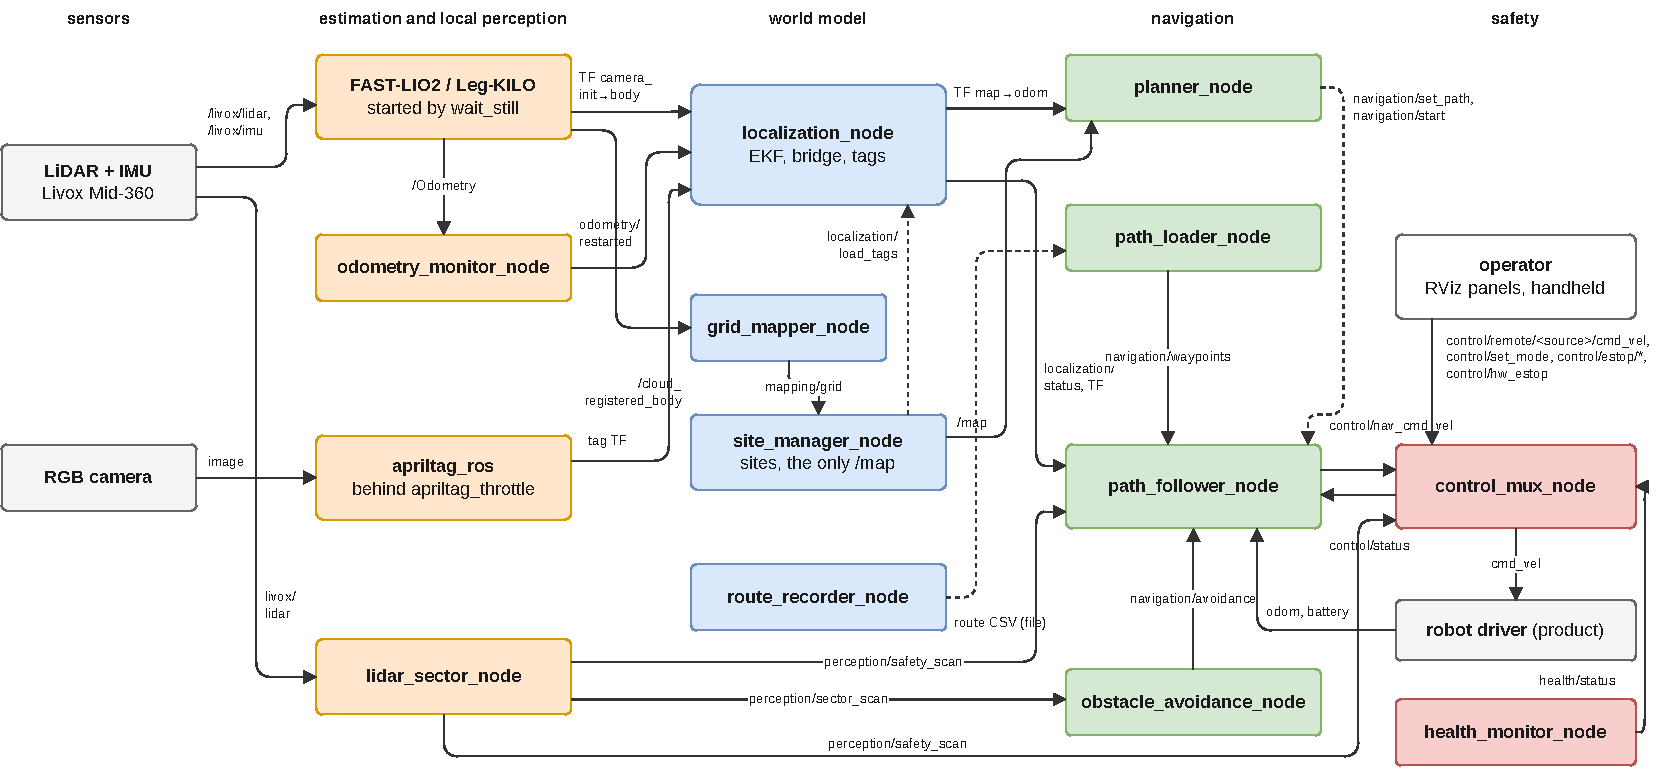
\includegraphics[width=\linewidth]{dataflow}
  \caption{Nodes and main topics. Solid: topics and TF; dashed: services and files.}
  \label{fig:dataflow}
\end{figure}
\end{landscape}

\begin{longtable}{@{}p{0.14\textwidth}p{0.36\textwidth}p{0.20\textwidth}p{0.20\textwidth}@{}}
  \toprule
  Package & Publishes & Subscribes & Services \\
  \midrule
  \endhead
  \bottomrule
  \endfoot
  odometry & \topic{odometry/status} (OdometryStatus, latched), \topic{odometry/restarted}
    (Empty) & \topic{/Odometry}, leg odometry, IMU & -- \\
  localization & TF \frm{map}$\to$\frm{odom} and the bridge (\frm{odom}$\to$\frm{camera_init},
    \frm{body}$\to$\frm{base_link}), \topic{localization/status} (latched),
    \topic{localization/pose} (PoseWithCovarianceStamped), \topic{localization/tag_markers} &
    \topic{odometry/restarted}, \topic{/initialpose}, IMU, \topic{/map} and the registered cloud
    (scan matching) & \topic{localization/start}, \topic{reset}, \topic{assume_origin},
    \topic{record_tags}, \topic{load_tags} \\
  perception & \topic{perception/sector_scan} (front), \topic{perception/safety_scan} (360°),
    \topic{perception/obstacles} & Livox CustomMsg or PointCloud2, TF & -- \\
  mapping & \topic{/map} (latched, only publisher), \topic{mapping/grid},
    \topic{mapping/status}, \topic{site/status}, \topic{route/saved} & registered cloud,
    \topic{localization/status} & \topic{site/list}, \topic{site/load}, \topic{mapping/start},
    \topic{mapping/stop}, \topic{mapping/save}, \topic{route/start}, \topic{route/stop},
    \topic{route/mark_stop_point} \\
  navigation & \topic{planner/path}, \topic{planner/status}, \topic{planner/costmap},
    \topic{navigation/status}, \topic{navigation/stop_point}, \topic{navigation/path},
    \topic{navigation/waypoints}, \topic{navigation/avoidance}, \topic{control/nav_cmd_vel},
    markers & \topic{/map}, \topic{perception/*_scan}, \topic{control/status},
    \topic{localization/status}, battery, odom & \topic{planner/go_to}, \topic{planner/plan},
    \topic{planner/cancel}, \topic{navigation/set_path}, \topic{navigation/load_path},
    \topic{navigation/start}, \topic{stop}, \topic{pause}, \topic{resume} \\
  control & \topic{cmd_vel} (only publisher), \topic{control/status} (latched) &
    \topic{control/nav_cmd_vel}, \topic{control/remote/<source>/cmd_vel},
    \topic{perception/safety_scan}, \topic{control/estop_request}, \topic{control/hw_estop},
    \topic{health/status} & \topic{control/set_mode}, \topic{control/estop/engage},
    \topic{control/estop/release} \\
  health & \topic{health/status} (latched), \topic{diagnostics} & configured topics, status
    topics, TF & -- \\
\end{longtable}

\section{Frames}
\label{sec:frames}

\begin{figure}[h]
  \centering
  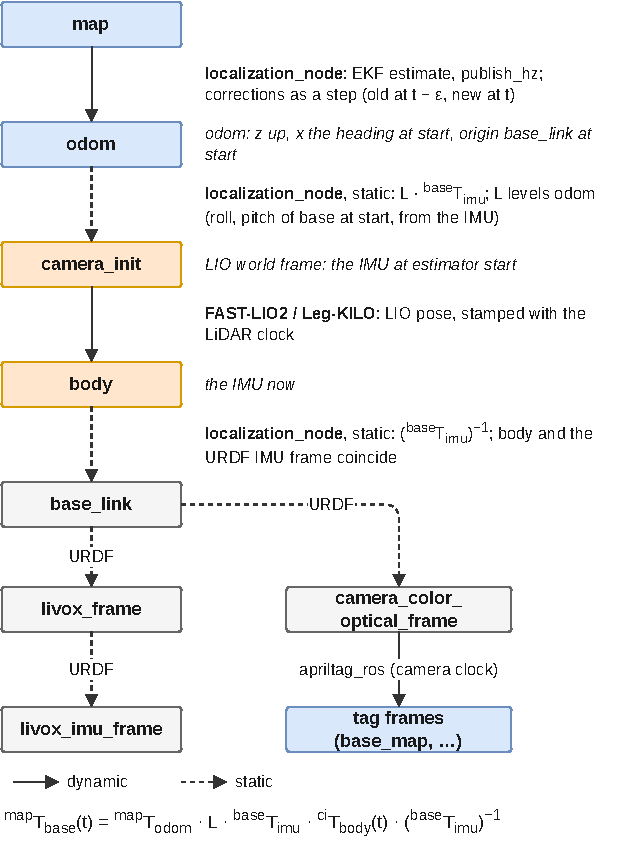
\includegraphics[width=0.62\textwidth]{tf_tree}
  \caption{TF tree and who publishes each edge.}
  \label{fig:tf}
\end{figure}

The tree follows REP-105 (Fig.~\ref{fig:tf}). The LiDAR-inertial estimator publishes
\frm{camera_init}$\to$\frm{body}: \frm{camera_init} is the IMU frame at estimator start and
\frm{body} the IMU now. Localization bridges it into the robot tree with two static transforms
and publishes the map correction:
\begin{equation}
  \T{map}{base}(t) = \T{map}{odom}\; \underbrace{L\, \T{base}{imu}}_{\T{odom}{ci}}\;
  \T{ci}{body}(t)\; \underbrace{\big(\T{base}{imu}\big)^{-1}}_{\T{body}{base}} .
  \label{eq:m-chain}
\end{equation}
$\T{base}{imu}$ is the URDF mounting of the IMU and $L$ the roll and pitch of the base at
estimator start (Section~\ref{sec:leveling}). Consequently \frm{odom} has $z$ against gravity,
its $x$ axis is the heading at start and its origin is \frm{base_link} at start. Frame names
come from \param{robot.frames.*}; the LIO frames are parameters of localization.

The edges with time-varying values are \frm{map}$\to$\frm{odom} (stamped by localization with
the node clock) and \frm{camera_init}$\to$\frm{body} (stamped by the estimator with the LiDAR
clock); everything else is static. This matters for the TF latency budget
(Section~\ref{sec:tf-budget}).

\section{Design principles}

\begin{enumerate}
  \item \textbf{One source of truth for the robot.} Every geometric and dynamic assumption is
    derived from the robot profile (Chapter~\ref{ch:config}); derived values are computed,
    never copied.
  \item \textbf{Pure core, ROS at the edge.} Algorithms are plain Python and numpy, unit-tested
    without ROS; nodes convert messages at the edge.
  \item \textbf{Plugins instead of if/elif.} Controllers and avoidance policies register in a
    named registry, open to entry points.
  \item \textbf{Uncertainty in the interfaces.} The robot pose is published with its
    covariance; statuses carry states, sigmas and reasons.
  \item \textbf{Safety independent of autonomy.} The safety layer only reads typed inputs and
    can be verified on its own; navigation pauses itself on the control status.
  \item \textbf{Fail safe.} Missing data is an obstacle; a failing callback stops the robot.
  \item \textbf{Compatibility.} SemVer; every package of the stack moves together across a
    breaking change.
\end{enumerate}

\section{Launch composition}

Each package has one launch file (\code{launch/<pkg>.launch.py}) with the arguments
\code{params_file}, \code{robot_params}, \code{use_sim_time} and \code{log_level}; parameters
are applied as \texttt{[package defaults, robot\_params, params\_file, non-empty overrides]}, so an
empty argument never overrides a value from a file. No package launch file includes another
one: the product bringup (generated from the template's \code{robot_bringup}) composes them.
Nodes that can plausibly crash set \code{respawn=True}; the robot driver must stop on its own
command timeout meanwhile.
